\section{Integers and Divisibility}

While $\Z$ is not closed under division (an integer divided by an integer is not always an integer), we can still come up with definitions for dividing integers. 

\begin{definition}{def3.1}
    If $a,b\in\Z$ and $a\ne 0$, then $a$ \textbf{divides} $b$ ($a|b$) if there exists an integer $k$ such that $ak = b$. In this case, $a$ is a \textbf{factor/divisor} of $b$, and $b$ is a \textbf{multiple} of $a$. If $a$ does not divide $b$, then the notation is $a \nmid b$.
\end{definition}

\begin{itemize}
    \item $2|10$ because $2(5)=10$ where $k=5$
    \item $4 \nmid 10$ because $\frac{10}{4} = 2.5$ which is not an integer
    \item $-6|42$ because $-6(-7)=42$ where $k=-7$
\end{itemize}


\begin{theorem}[The Divisibility Theorem]{theorem3.1:label}
    Let $a,b,c \in \Z$ where $a \ne 0$. Then the following statements are true:

    \begin{itemize}
        \item $a|a$
        \item $a|0$
        \item If $a|b$ and $a|c$, then $a|(b+c)$
        \item If $a|b$, then $a|bc$ for all integers $c$
        \item If $a|b$ and $b|c$, then $a|c$
    \end{itemize}
\end{theorem}

\begin{corollary}[Corollary to the Divisibility Theorem]{cor3.1:label}
    Let $a,b,c\in \Z$ where $a\ne 0$. If $a|b$ and $b|c$, then $a | (mb + nc)$ for all integers $m$ and $n$.
\end{corollary}

\subsection{The Division Algorithm}

\begin{itemize}
    \item Let $a \in \Z$ and $d \in \Z^+$
    \item There are unique integers $q$ and $r$ such that $a = dq + r$ where $0 \le r < d$
    \item $a$ is the \textit{dividend}
    \item $d$ is the \textit{divisor}
    \item $q$ is the \textit{quotient}
    \item $r$ is the remainder 
\end{itemize}

\textbf{THE $\div$ OPERATION:} $a \div b$ means divide $b$ by $a$ and leave off the remainder. 

\begin{itemize}
    \item EX: $4 \div 10 = 2$ because $\frac{10}{4} = 2.5$ and we just care about the whole number part of the answer and disregard the remainder.
\end{itemize}

\textbf{THE $\mod$ OPERATOR:} $a \mod b$ means divide $b$ by $a$ and leave JUST the remainder.

\begin{itemize}
    \item EX: $4 \mod 10 = 2$ because $\frac{10}{4} = 2\text{ R}2$ and we just care about the remainder part of the answer (2)
\end{itemize}

\begin{problem}
    If 100 is divided by 23, write as $a=dq+r$ and find the quotient and remainder.

    $$
    \begin{aligned}
        100 &= 23q + r\\
        100 &= 23 \cdot 4 + 8\\
        100 \div 23 = 4\\
        100 \mod 23 = 8
    \end{aligned}
    $$
\end{problem}

\begin{problem}
    If -100 is divided by 23, write as $a=dq+r$ and find the quotient and remainder.

    $$
    \begin{aligned}
        -100 &= 23q + r
        -100 &= 23(-4) + (-8)\\
        \text{remainder can't be negative so we add another factor of 23 to make the remanider positive}
        -100 &= 23(-5) + 15\\
        -100 \div 23 = -5\\
        -100 \mod 23 = 15
    \end{aligned}
    $$
\end{problem}


\subsection{Introduction to Congruence}

\begin{definition}[Modular Congruence]{def3.2:label}
    Let $a$ and $b$ be integers and let $n$ be a positive integer. Then $a$ and $b$ are \textbf{congruent modulo $n$} if $n|(a-b)$. If $a$ and $b$ are congruent moduo $n$, we then write that $a \equiv b (\mod n)$
\end{definition}

\textbf{NOTE:} $a$ and $b$ are congruent modulo $n$ when the have the same remainder when divided by $n$. This means that if $a$ and $b$ are congruent modulo $n$, then $a \mod n = b \mod n$.

\begin{itemize}
    \item $12 \equiv 2 \mod 5$ because $12 \mod 5 = 2 = 2 \mod 5$
    \item $-7 \not\equiv 2 \mod 5$ because $-7 \mod 5 = 3 \ne 2 \mod 5$
\end{itemize}

\textbf{NOTE:} $\{5k + 2 | k \in \Z\}$ is the set of numbers congruent to a modulo $n$



\section{Integer Representations and Algorithms}

\subsection{Integers in Different Bases}

\begin{theorem}[Integers in Differen Bases]{theorem3.2:label}
    Let $b \in \Z$ and $b > 1$. Then if $n \in \Z^+$, it has a unique base-$b$ expansion, expressed uniquely in the form:

    $$
    n = a_kb^k + a_{k-1}b^{k+1} + \cdots + a_1b^1 + a_0
    $$

    Where $k$ is a non-negative integer and $a_0,a_1,a_2,\cdots,a_k$ are all non-negative integers that are less than $b$ and $a_k \ne 0$.
\end{theorem}

\begin{itemize}
    \item We denote what base we are in by using a subscript equivalent to the base: $(a_ka_{k-1}...a_1a_0)_b$
    \item $b = 10$ is \textit{decimal} expansion
    \item $b = 2$ is \textit{binary} expansion
    \item $b=8$ is the \textit{octal} expansion
    \item $b = 16$ is the \textit{hexaedcimal} expansion
\end{itemize}

\begin{problem}
    Convert $(10010111)_2$ to decimal.

    $$
    \begin{aligned}
        (10010111)_2 &= 1 \cdot 2^7 + 0 \cdot 2 ^6 + 0 \cdot 2 ^5 + 1 \cdot 2 ^4 + 0 \cdot 2 ^3 + 1 \cdot 2 ^2 + 1 \cdot 2 ^1 + 1 \cdot 2 ^0\\
        &= 128 + 16 + 4 + 2 + 1\\
        &= 151
    \end{aligned}
    $$
\end{problem}


\begin{problem}
    Convert $(A1F)_{16}$ to decimal.
\end{problem}


\begin{problem}
    Convert $(1036)_8$ to decimal.
\end{problem}


\subsection{Converting From Base-10 to Base-$n$}


To convert a number from base-10 to base-$n$, you repeatedly use the division algorithm in the following way:

$$
\begin{aligned}
    n &= bq_0 + r_0\\
    q_0 &= bq_1 + r_1\\
    q_1 &= bq_2 + r_2\\
    &...\\
    q_{k-1} = bq_k + r_k
\end{aligned}
$$

You stop this process when $q_k$ is equal to 0. Then, the number in base $n$ is the list of all $r_n$ (all the remainders) in reverse order (so from the bottom step remainder to the first step remainder).

\begin{problem}
    Convert $(108)_10$ into the following bases:

    \begin{itemize}
        \item Binary:
        \item Octal:
        \item Hexadecimal:
    \end{itemize}
\end{problem}


\subsection{Converting From Base-$n$ to Base-$m$}

Every three digits in binary correspond to one octal digit. Similarly, every four digits in binary correspond to one hexadecimal digit.\\

On the next page, you can see a chart matching all of the base 10 numbers from 0-16 and what each number's binary, octal, and hexadecimal representations are. You can then use this table to convert any number in base 2,4,8,16 to base 2,4,8,16.\newpage

\begin{center}
    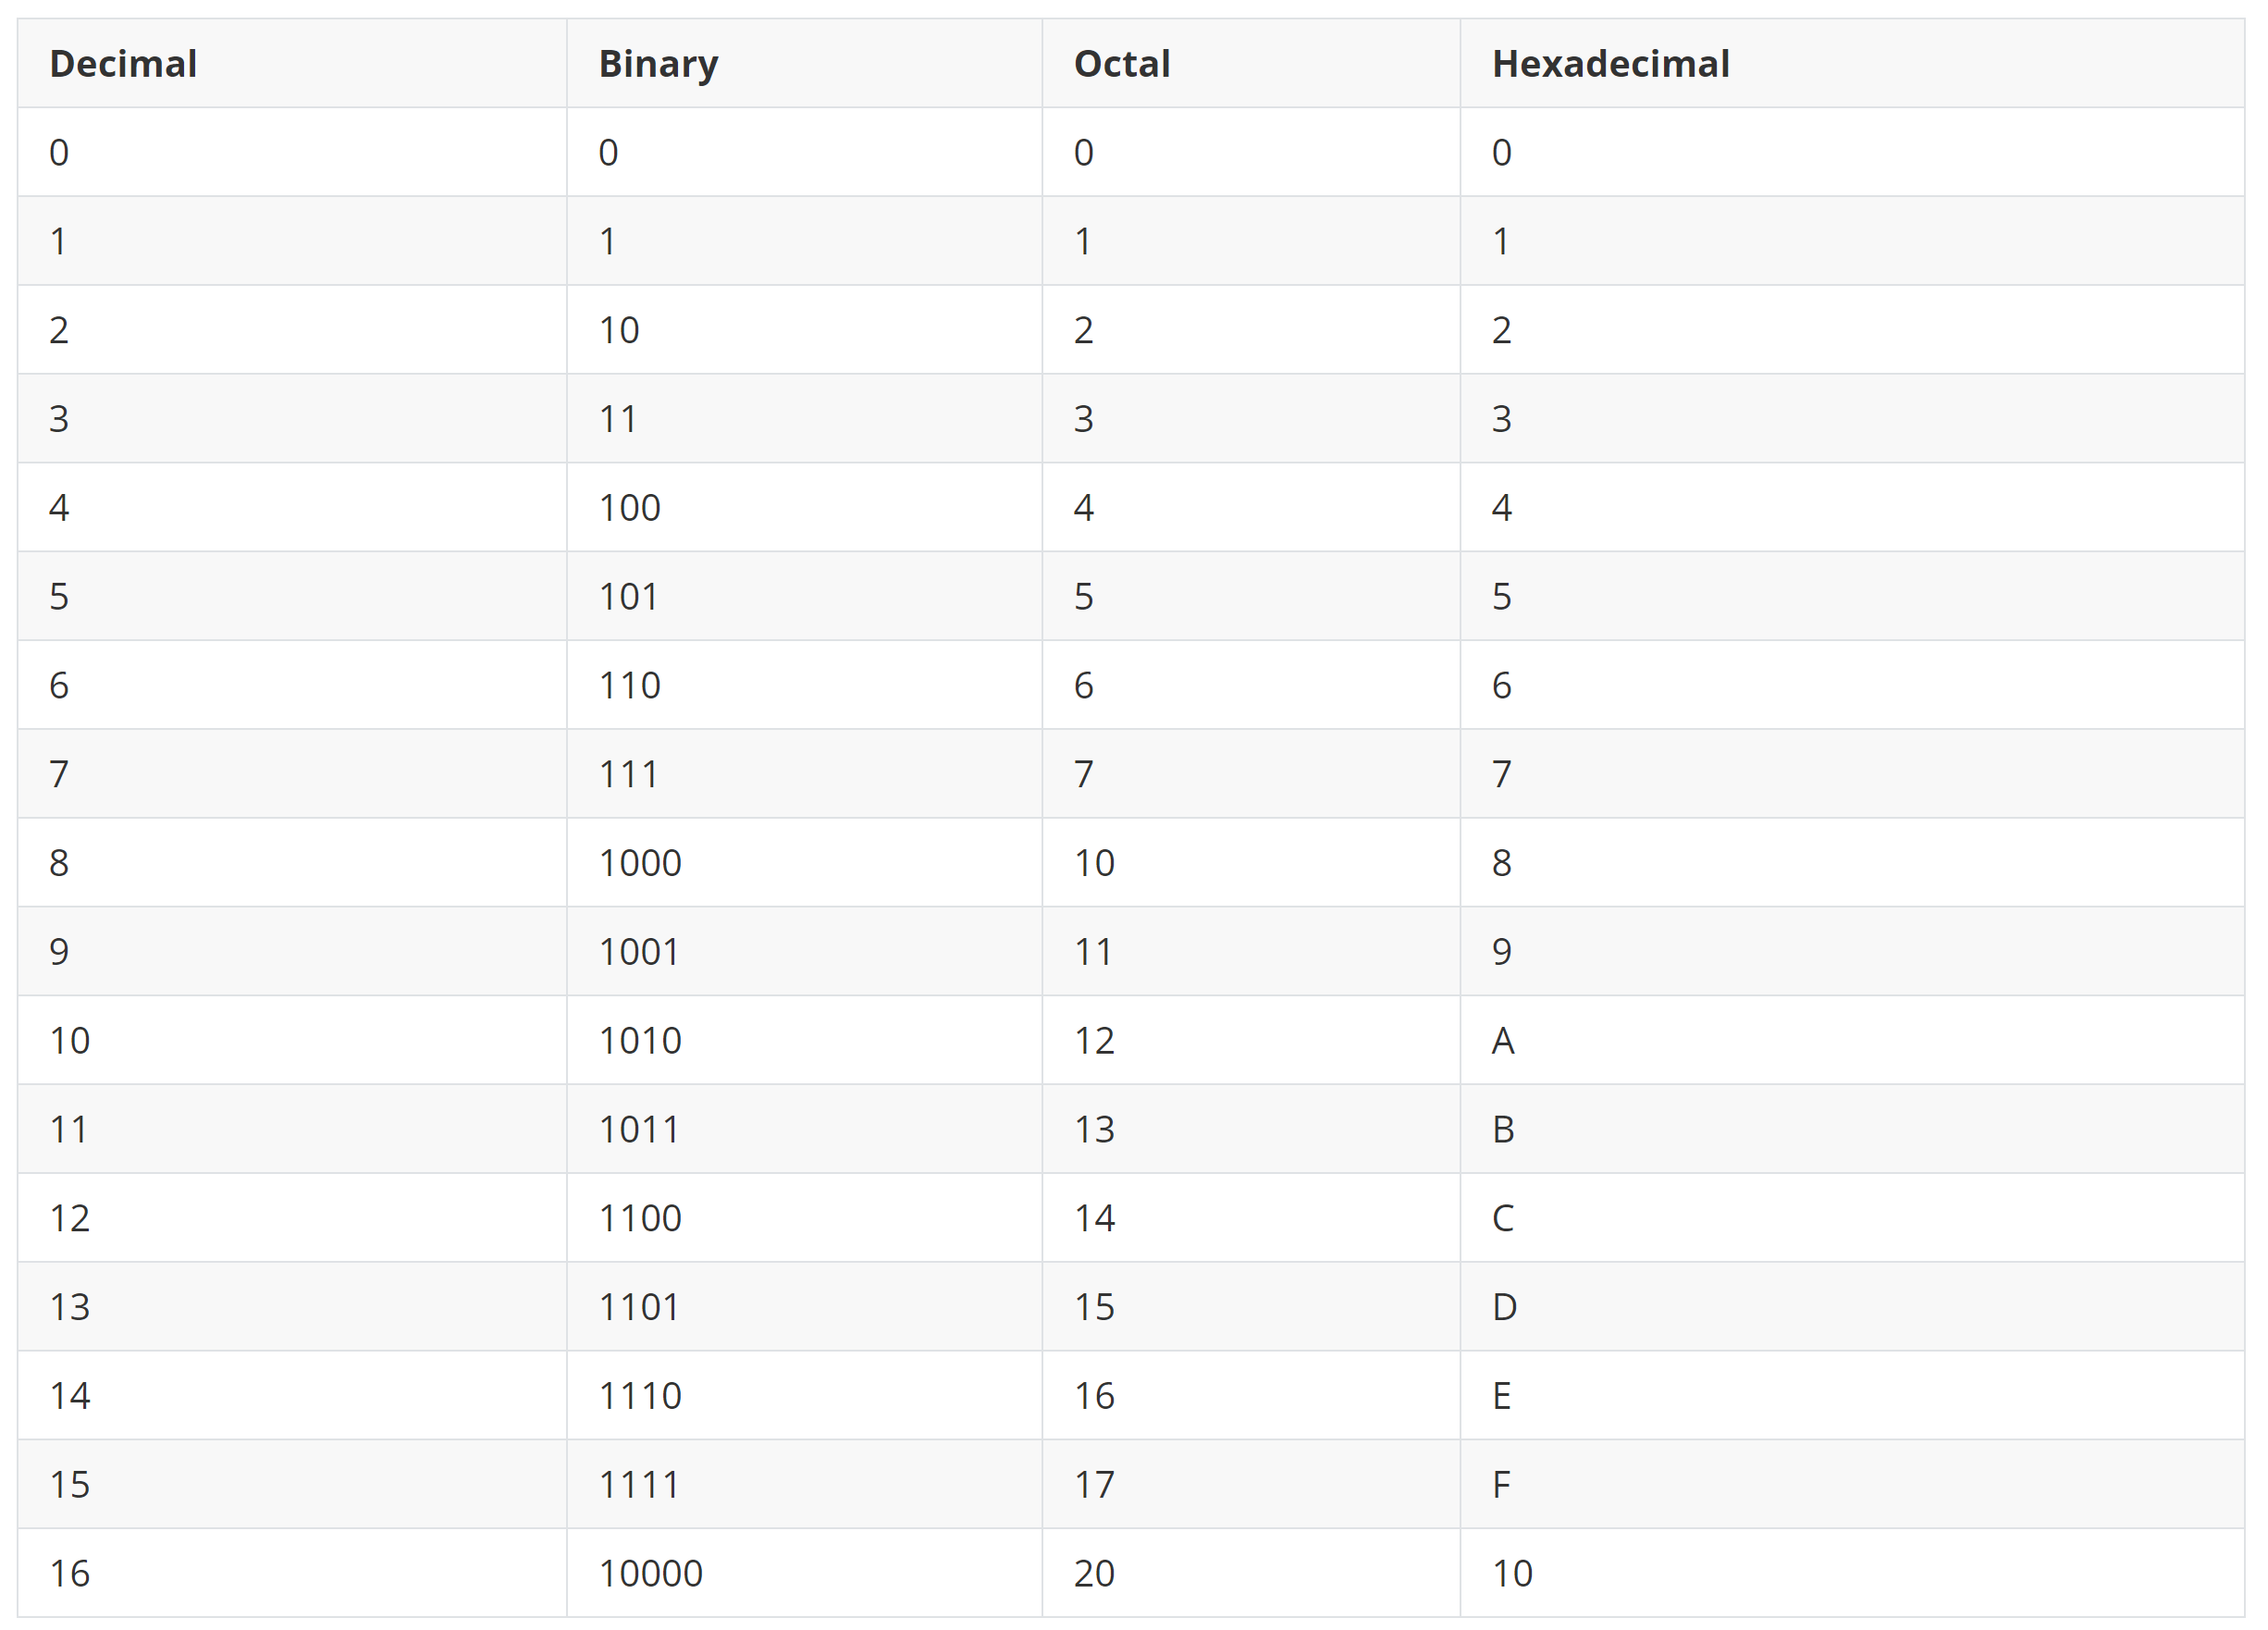
\includegraphics[width=1.2\textwidth]{chapters/ch3/images/Number_Chart.PNG}
\end{center}

\begin{problem}
    Convert $(DB5)_{16}$ into binary and octal.
\end{problem}


\section{Primes and Greatest Common Divsors}

\begin{definition}[Prime Numbers]{def3.3.1:label}
    An integer $p$ greater than 1 is \textbf{prime} if the only positive factors of $p$ are 1 and $p$.
\end{definition}

\begin{theorem}[The Fundamental Theorem of Arithmetic]{theorem3.3.1:label}
    Every integer greater than 1 can be written uniquely as a prime or as the prodct of two or more primes written in increasing order.
\end{theorem}

\begin{problem}
    Fnid the prime factorizations of the following numbers:

    \begin{itemize}
        \item $36 = 6^2 = (2\cdot 3)^2 = 2^2\cdot 3^2$\\
        \item $84 = 7 \cdot 12 = 7 \cdot 3 \cdot 2 \cdot 2 = 2^2\cdot 3 \cdot 7$
        \item $31 = 31 \cdot 1$
    \end{itemize}
\end{problem}

\begin{proposition}{prop3.3.1:label}
    If $n$ has a prime divisor, then it must have one that is less than or equal to $\sqrt{n}$
\end{proposition}

Listed below is a table with all of the primes that are $\le 100$. Every number that is \textbf{bold} is a prime number.

\begin{center}
    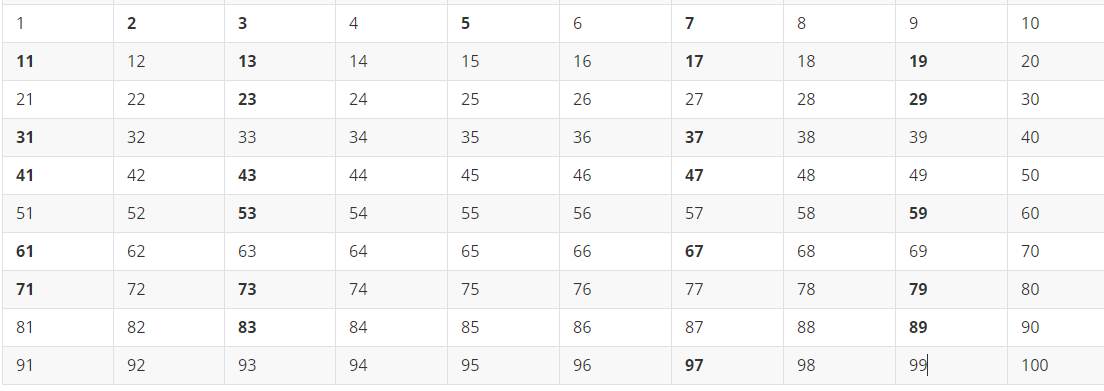
\includegraphics[width=1.2\textwidth]{chapters/ch3/images/Primes_Chart.PNG}
\end{center}


\begin{theorem}{3.3.2:label}
    There are infinietly many primes.
\end{theorem}

\begin{definition}{3.3.2:label}
    Let $a$ and $b$ be integers with $a$ and $b$ not being equal to 0. The largest integer $d$ such that $d|a$ and $d|b$ is called the \textbf{greatest common divisor} of $a$ and $b$. The notation is $\gcd(a,b)$
\end{definition}

\begin{problem}
    Find $\gcd(36,84).$

    $$
    \begin{aligned}
        36 &= 6 \cdot 6 = 2^2 \cdot 3^2\\
        84 &= 7 \cdot 12 = 2^2 cdot 3 \cdot 7\\
        \gcd(36,84) &= 2^2 \cdot 3 = 12
    \end{aligned}
    $$
\end{problem}

\begin{problem}
    Find $\gcd(9,49).$

    $$
    \begin{aligned}
        9 &= 3^2\\
        49 &= 7^2\\
        \gcd(9,49) &= 1
    \end{aligned}
    $$
\end{problem}


\begin{definition}[Relatively Prime]{def3.3.3:label}
    Two integers $a$ and $b$ are \textbf{relatively prime} if $\gcd(a,b) = 1$.
\end{definition}


\begin{definition}{def3.3.4:label}
    The least common multiple of the positive integers $a$ and $b$ is is the smallest positive integer that is divisible by both $a$ and $b$. Notation is $\lcm(a,b)$.
\end{definition}